\documentclass[11pt]{article}
\usepackage{amsmath, amssymb, amsthm}
\usepackage{geometry}
\usepackage{enumitem}
\usepackage{hyperref}
\usepackage{mathtools}
\usepackage{tikz}
\geometry{margin=1in}
% theorem environments
\newtheorem{theorem}{Theorem}[section]
\newtheorem{lemma}[theorem]{Lemma}
\newtheorem{corollary}[theorem]{Corollary}
\theoremstyle{definition}
\newtheorem{definition}[theorem]{Definition}
\theoremstyle{remark}
\newtheorem{remark}[theorem]{Remark}
\usepackage{hyperref}
\hypersetup{
    colorlinks=true,
    linkcolor=blue,
    filecolor=magenta,      
    urlcolor=cyan,
}

\title{Chapter 5 --- Matchings \\}
\author{Luca De Vecchis}
\date{Jan 2026}

\begin{document}
\maketitle
\tableofcontents
\newpage

\section{Preliminaries and Notation}

Let $G = (V,E)$ be a finite graph.  
For $v \in V$, denote by $d(v)$ the degree of $v$.  
For $S \subseteq V$, let $G - S$ denote the induced subgraph obtained by deleting $S$ and all incident edges.

\section{Matchings}

\begin{definition}[Matching]
A \emph{matching} in $G$ is a set $M \subseteq E$ such that
\begin{align*}
\forall e,f \in M, \quad e \neq f \;\Rightarrow\; e \cap f = \varnothing .
\end{align*}
\end{definition}

\begin{definition}
Let $M$ be a matching.
\begin{itemize}
    \item A vertex $v$ is \emph{matched} if $\exists e \in M$ such that $v \in e$
    \item Otherwise, $v$ is \emph{free}
\end{itemize}
\end{definition}

\begin{definition}[Maximum and Perfect Matchings]
M is:
\begin{itemize}
    \item $M$ is \emph{maximum} if $|M| \ge |M'|$ for all matchings $M'$.
    \item $M$ is \emph{perfect} if every vertex of $G$ is matched.
\end{itemize}
\end{definition}

\section{Matchings and Coverings in Bipartite Graphs}

Let $G = (X \cup Y, E)$ be a bipartite graph.

\subsection{Vertex Covers}

\begin{definition}[Vertex Cover]
A \emph{vertex cover} of $G$ is a set $C \subseteq V(G)$ such that every edge in $E$ is incident to at least one vertex in $C$.
\end{definition}

\begin{definition}[Minimum Vertex Cover]
A \emph{minimum vertex cover} is a vertex cover of smallest possible cardinality. Denote its size by $\tau(G)$.
\end{definition}
\clearpage

\subsection{Relationship with Matchings}

\begin{theorem}[K\H{o}nig's Min--Max Theorem]
In any bipartite graph $G$,
\[
\nu(G) = \tau(G),
\]
where $\nu(G)$ is the size of a maximum matching and $\tau(G)$ is the size of a minimum vertex cover.
\end{theorem}

\begin{proof}[Sketch]
Let $M$ be a maximum matching.  
Let $Z$ be the set of vertices reachable from free vertices in $X$ via alternating paths.  
Define 
\[
C = (X \setminus Z) \cup (Y \cap Z).
\]

\paragraph*{Cover property.} Every edge is incident to at least one vertex in $C$.  

\paragraph*{Cardinality.} Each edge of $M$ contributes exactly one vertex to $C$, so $|C| = |M| = \nu(G)$.
\end{proof}

\begin{remark}
This theorem establishes a min--max relation between matchings and covers in bipartite graphs. It is not true for general graphs.
\end{remark}

\subsection{K-Regular Bipartite Graphs}

\begin{definition}[K-Regular Bipartite Graph]
A bipartite graph $G = (X \cup Y, E)$ is \emph{$k$-regular} if every vertex has degree $k$, i.e.,
\[
d(v) = k \quad \forall v \in X \cup Y.
\]
\end{definition}

\begin{theorem}
Every $k$-regular bipartite graph has a perfect matching.
\end{theorem}

\begin{proof}[Sketch]
Use Hall's theorem. For any $S \subseteq X$,
\[
|N(S)| \ge \frac{k |S|}{k} = |S|,
\]
so the Hall condition is satisfied. Hence, a matching saturating $X$ exists. Since $|X| = |Y|$, it is a perfect matching.
\end{proof}

\subsection{Coverings and Matchings Formulas}

\begin{itemize}
    \item Maximum matching: $\nu(G) = \max\{|M| : M \text{ is a matching in } G\}$
    \item Minimum vertex cover: $\tau(G) = \min\{|C| : C \text{ is a vertex cover in } G\}$
    \item For bipartite graphs: $\nu(G) = \tau(G)$ (K\H{o}nig)
\end{itemize}
\clearpage

\section{Alternating Structure and Auxiliary Graphs}

\begin{figure}[h]
\centering
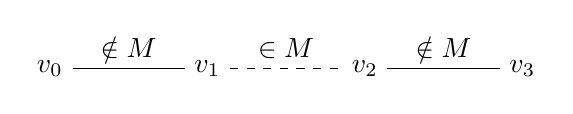
\begin{tikzpicture}
\node (v0) at (0,0) {$v_0$};
\node (v1) at (2,0) {$v_1$};
\node (v2) at (4,0) {$v_2$};
\node (v3) at (6,0) {$v_3$};

\draw (v0) -- node[above] {$\notin M$} (v1);
\draw[dashed] (v1) -- node[above] {$\in M$} (v2);
\draw (v2) -- node[above] {$\notin M$} (v3);
\end{tikzpicture}
\caption{An alternating path with respect to a matching $M$.}
\end{figure}

\subsection{Auxiliary Graph}

Given a matching $M$, define an orientation of $E$ by
\[
xy \in E \quad \longrightarrow \quad
\begin{cases}
x \to y, & xy \notin M, \\
y \to x, & xy \in M .
\end{cases}
\]

This orientation encodes alternating paths as directed paths.

\subsection{Alternating and Augmenting Paths}

\begin{definition}[Alternating Path]
A path $P = v_0 v_1 \dots v_k$ is \emph{alternating with respect to $M$} if
\[
v_{i-1}v_i \in M
\;\Longleftrightarrow\;
v_iv_{i+1} \notin M
\quad \text{for all admissible } i .
\]
\end{definition}

\begin{definition}[Augmenting Path]
An alternating path whose endpoints $v_0$ and $v_k$ are free vertices.
\end{definition}

\begin{lemma}
If $P$ is an augmenting path relative to $M$, then
\[
|M \triangle E(P)| = |M| + 1 .
\]
\end{lemma}

\begin{proof}
Along $P$, the number of edges not in $M$ exceeds the number of edges in $M$ by one,
since both endpoints of $P$ are free. The replacement of the edges of $M \cap E(P)$ with those of $E(P) \setminus M$ therefore increases the size of the matching by exactly one.
\end{proof}


\section{Symmetric Difference of Matchings}

\begin{definition}
For matchings $M$ and $M'$, define the symmetric difference
\[
M \triangle M'
=
(M \setminus M') \cup (M' \setminus M) .
\]
\end{definition}

\begin{lemma}
Each connected component of $(V, M \triangle M')$ is either
\begin{itemize}
    \item an even cycle alternating between $M$ and $M'$, or
    \item an alternating path.
\end{itemize}
\end{lemma}

\begin{corollary}
If $|M'| > |M|$, then $M \triangle M'$ contains an augmenting path with respect to $M$.
\end{corollary}

\begin{proof}
Even alternating cycles contribute equally to both matchings.
Since $|M'| > |M|$, there must exist an alternating path containing more edges of $M'$
than of $M$, which is necessarily an augmenting path relative to $M$.
\end{proof}


\section{Berge's Theorem}

\begin{theorem}[Berge]
A matching $M$ is maximum if and only if there exists no augmenting path relative to $M$.
\end{theorem}

\begin{remark}
Berge’s theorem provides a complete optimality criterion for matchings and underlies all matching algorithms.
\end{remark}

\paragraph*{Necessity.}
If an augmenting path exists relative to $M$, then replacing matched edges along this path
produces a larger matching, contradicting maximality.
\paragraph*{Sufficiency.}
Assume $M$ is not maximum. Then there exists a matching $M'$ with $|M'| > |M|$.
By the symmetric difference argument, $M \triangle M'$ contains an augmenting path,
contradicting the assumption.

\begin{figure}[h]
\centering
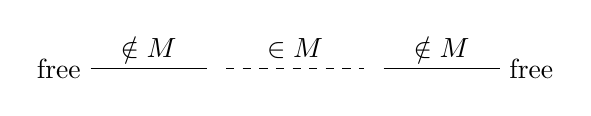
\begin{tikzpicture}
\node (f1) at (0,0) {free};
\node (u) at (2,0) {};
\node (v) at (4,0) {};
\node (f2) at (6,0) {free};

\draw (f1) -- node[above] {$\notin M$} (u);
\draw[dashed] (u) -- node[above] {$\in M$} (v);
\draw (v) -- node[above] {$\notin M$} (f2);
\end{tikzpicture}
\caption{An augmenting path.}
\end{figure}

\section{Bipartite Graphs}

\begin{definition}
A graph $G = (X \cup Y, E)$ is \emph{bipartite} if
\[
E \subseteq X \times Y .
\]
\end{definition}

\subsection{Neighborhood Function}

\begin{definition}
For $S \subseteq X$, define
\[
N(S) = \{\, y \in Y \mid \exists x \in S \text{ such that } xy \in E \,\}.
\]
\end{definition}

\section{Hall's Theorem (Marriage Theorem)}

\begin{theorem}[Hall]
A bipartite graph $(X,Y)$ has a matching saturating $X$ if and only if
\[
\forall S \subseteq X, \qquad |N(S)| \ge |S| .
\]
\end{theorem}

\paragraph*{Necessity.}
If a matching saturates $X$, then each vertex of $S \subseteq X$ is matched to a distinct
vertex of $Y$. Hence $|N(S)| \ge |S|$.

\paragraph*{Sufficiency.}
Assume Hall’s condition holds and proceed by induction on $|X|$.

If $|X| = 1$, the result is trivial. Otherwise, one of the following holds:
\begin{itemize} 
\item There exists a nonempty $S \subsetneq X$ such that $|N(S)| = |S|$.
    Apply induction to the induced bipartite graphs
    $(S,N(S))$ and $(X \setminus S, Y \setminus N(S))$
    and combine the resulting matchings.
    \item For every nonempty $S \subseteq X$, we have $|N(S)| \ge |S| + 1$.
    Remove any vertex $x \in X$ and apply induction to $X \setminus \{x\}$.
\end{itemize}

\section{K\H{o}nig's Theorem}

\begin{theorem}[K\H{o}nig]
For any bipartite graph $G$,
\[
\nu(G) = \tau(G),
\]
where $\nu(G)$ is the size of a maximum matching and $\tau(G)$ is the size of a minimum vertex cover.
\end{theorem}

\begin{proof}[Proof sketch]
Let $M$ be a maximum matching.
Let $Z$ denote the set of vertices reachable from free vertices in $X$
by alternating paths and define
\[
C = (X \setminus Z) \cup (Y \cap Z).
\]

\paragraph*{Vertex cover.}
Every edge is incident to at least one vertex in $C$, otherwise an alternating path
could be extended, contradicting maximality.

\paragraph*{Cardinality.}
Each edge of $M$ contributes exactly one vertex to $C$, hence $|C| = |M|$.

Therefore $\tau(G) = \nu(G)$.
\end{proof}


\section{Tutte's Theorem}

\begin{theorem}[Tutte]
A graph $G$ has a perfect matching if and only if
\[
\forall S \subseteq V(G), \qquad o(G-S) \le |S| ,
\]
where $o(G-S)$ is the number of odd components of $G-S$.
\end{theorem}

\paragraph*{Necessity.}
Let $M$ be a perfect matching and $S \subseteq V(G)$.
Each odd component of $G-S$ must contain a vertex matched into $S$.
Thus $o(G-S) \le |S|$.

\paragraph*{Sufficiency.}
Assume the condition holds for all subsets $S$.
Using the Tutte--Berge construction, the problem is reduced to a bipartite matching
instance to which Hall’s theorem applies, yielding a perfect matching of $G$.
\clearpage

\section{Algorithms}

\subsection{Hopcroft--Karp Algorithm}

The Hopcroft--Karp algorithm finds a \emph{maximum matching} in a bipartite graph efficiently.

\paragraph*{Input.} Bipartite graph $G = (X \cup Y, E)$.

\paragraph*{Overview.} The algorithm repeatedly searches for a maximal set of \emph{vertex-disjoint shortest augmenting paths} and augments along all of them simultaneously.

\paragraph*{Procedure.}
\begin{enumerate}
    \item Initialize $M = \emptyset$.
    \item While there exists an augmenting path:
    \begin{itemize}
        \item Use BFS to compute \emph{layered graphs} from free vertices in $X$ to free vertices in $Y$.
        \item Use DFS to find a maximal set of vertex-disjoint shortest augmenting paths in the layered graph.
        \item Augment $M$ along all these paths.
    \end{itemize}
\end{enumerate}

\paragraph*{Time Complexity.} $O\!\left(\sqrt{|V|}\, |E|\right)$.

\paragraph*{Remarks.}  
By augmenting along multiple disjoint paths simultaneously, the algorithm reduces the number of augmentation rounds and achieves sublinear time per round compared to naive augmenting path algorithms.

\subsection{Kuhn--Munkres Algorithm (Hungarian Method)}

The Kuhn--Munkres algorithm solves the \emph{optimal assignment problem} in a complete bipartite graph with weight function
\[
w : X \times Y \to \mathbb{R}.
\]

\paragraph*{Goal.} Find a perfect matching $M$ maximizing $\sum_{(x,y) \in M} w(xy)$ \\
(or minimizing costs $c_{ij}$ in the OAP).

\paragraph*{Step 0: Initial feasible vertex labeling.}  
Assign a function $l : X \cup Y \to \mathbb{R}$ such that
\[
l(x) + l(y) \ge w(xy) \quad \forall x \in X, y \in Y.
\]
Define the \emph{equality graph} $G_l$ as
\[
G_l = \{ (x,y) \in X \times Y : l(x) + l(y) = w(xy) \}.
\]

\noindent Choose an arbitrary matching $M$ in $G_l$.

\paragraph*{Step 1: Check for optimality.}  
If $M$ saturates $X$ (and $|X| = |Y|$), then $M$ is a perfect matching. By the \emph{Optimal Assignment Theorem (5.5)}, $M$ is an optimal matching. Otherwise, select an $M$-unsaturated vertex $u \in X$, and set
\[
S = \{ u \}, \quad T = \emptyset.
\]

\paragraph*{Step 2: Construct alternating tree.}  
While $N(S) \neq T$ in the equality graph $G_l$:
\begin{enumerate}[label=(\alph*)]
    \item Compute
    \[
    \alpha = \min \{\, l(x) + l(y) - w(xy) \mid x \in S, y \notin T \,\}.
    \]
    \item Update the feasible labeling $l$ to $f$:
    \[
    f(v) =
    \begin{cases}
        l(v) - \alpha, & v \in S, \\
        l(v) + \alpha, & v \in T, \\
        l(v), & \text{otherwise}.
    \end{cases}
    \]
    \item Update $G_l$ to the new equality graph $G_f$.
\end{enumerate}

\paragraph*{Step 3: Augment matching.}  
Once a free vertex $y \in Y$ is reachable in the equality graph, construct an alternating path from $u$ to $y$ and augment $M$. Repeat the procedure until $M$ saturates $X$.

\paragraph*{Remarks.}  
\begin{itemize}
    \item $\alpha > 0$ ensures progress by increasing the size of the equality graph while maintaining feasibility.
    \item Each iteration preserves the \emph{feasible vertex labeling property} $l(x) + l(y) \ge w(xy)$.
    \item Time complexity is $O(n^3)$ for $|X| = |Y| = n$.
\end{itemize}
\clearpage

\section{Illustration: The Hungarian Method}

The following matrices and graphs illustrate the process of finding an optimal assignment by adjusting vertex labels to find a perfect matching in the equality subgraph.

\begin{figure}[h]
    \centering
    % Matrix (a) and (b)
    \begin{minipage}{0.45\textwidth}
        \centering
        \[ (a) \quad \begin{bmatrix} 3 & 5 & 5 & 4 & 1 \\ 2 & 2 & 0 & 2 & 2 \\ 2 & 4 & 4 & 1 & 0 \\ 0 & 1 & 1 & 0 & 0 \\ 1 & 2 & 1 & 3 & 3 \end{bmatrix} \]
        \vspace{1cm}
        \[ (b) \quad \begin{bmatrix} 3 & 5 & 5 & 4 & 1 \\ 2 & 2 & 0 & 2 & 2 \\ 2 & 4 & 4 & 1 & 0 \\ 0 & 1 & 1 & 0 & 0 \\ 1 & 2 & 1 & 3 & 3 \end{bmatrix} 
        \begin{matrix} 5 \\ 2 \\ 4 \\ 1 \\ 3 \end{matrix} \]
        \hspace{0.5cm} $0 \quad 0 \quad 0 \quad 0 \quad 0$
    \end{minipage}
    \hfill
    % Graph (c)
    \begin{minipage}{0.45\textwidth}
        \centering
        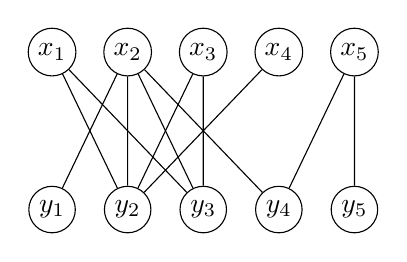
\begin{tikzpicture}[scale=0.8, every node/.style={circle, draw, inner sep=2pt}]
            \foreach \i in {1,...,5} {
                \node (x\i) at (\i*1.2, 2.5) {$x_{\i}$};
                \node (y\i) at (\i*1.2, 0) {$y_{\i}$};
            }
            \draw (x1)--(y2) (x1)--(y3);
            \draw (x2)--(y1) (x2)--(y2) (x2)--(y3) (x2)--(y4);
            \draw (x3)--(y2) (x3)--(y3);
            \draw (x4)--(y2);
            \draw (x5)--(y4) (x5)--(y5);
        \end{tikzpicture}
        \\ (c)
    \end{minipage}

    \vspace{1cm}

    % Matrix (d) and Graph (e)
    \begin{minipage}{0.45\textwidth}
        \centering
        \[ (d) \quad \begin{bmatrix} 3 & 5 & 5 & 4 & 1 \\ 2 & 2 & 0 & 2 & 2 \\ 2 & 4 & 4 & 1 & 0 \\ 0 & 1 & 1 & 0 & 0 \\ 1 & 2 & 1 & 3 & 3 \end{bmatrix} 
        \begin{matrix} 4 \\ 2 \\ 3 \\ 0 \\ 3 \end{matrix} \]
        \hspace{0.5cm} $0 \quad 1 \quad 1 \quad 0 \quad 0$
    \end{minipage}
    \hfill
    \begin{minipage}{0.45\textwidth}
        \centering
        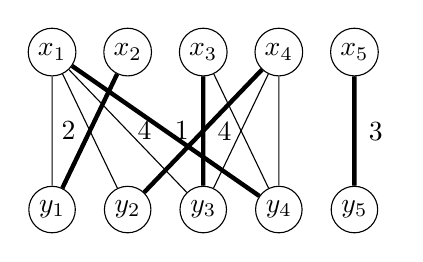
\begin{tikzpicture}[scale=0.8, every node/.style={circle, draw, inner sep=2pt}]
            \foreach \i in {1,...,5} {
                \node (x\i) at (\i*1.2, 2.5) {$x_{\i}$};
                \node (y\i) at (\i*1.2, 0) {$y_{\i}$};
            }
            % Edges
            \draw (x1)--(y1) (x1)--(y2) (x1)--(y3) (x1)--(y4);
            \draw (x2)--(y1);
            \draw (x3)--(y3) (x3)--(y4);
            \draw (x4)--(y2) (x4)--(y3) (x4)--(y4);
            \draw (x5)--(y5);
            % Matching (Thick edges)
            \draw[ultra thick] (x1)--(y4) node[midway, left, draw=none] {4};
            \draw[ultra thick] (x2)--(y1) node[midway, left, draw=none] {2};
            \draw[ultra thick] (x3)--(y3) node[midway, right, draw=none] {4};
            \draw[ultra thick] (x4)--(y2) node[midway, left, draw=none] {1};
            \draw[ultra thick] (x5)--(y5) node[midway, right, draw=none] {3};
        \end{tikzpicture}
        \\ (e)
    \end{minipage}
    \caption{The Kuhn-Munkres algorithm: from weight matrix to optimal matching.}
\end{figure}


\end{document}
